\documentclass[10pt]{article}

\usepackage{mathtools}
\usepackage{amsmath}
\usepackage{amssymb}
\usepackage{color}
\usepackage{fullwidth}
\usepackage{graphicx}
\usepackage[margin=0.6in]{geometry}
\usepackage{tikz}
\usepackage{soul}
\usepackage{float}
\usepackage[hidelinks, urlcolor=blue, linkcolor=blue, colorlinks=true]{hyperref} 

\DeclarePairedDelimiterX\set[1]\lbrace\rbrace{\def\given{\;\delimsize\vert\;}#1}

\newcommand{\bcent}{\begin{center}}
\newcommand{\ecent}{\end{center}}
\newcommand{\tb}{\textbf}
\newcommand{\noin}{\noindent}
\newcommand{\benum}{\begin{enumerate}}
\newcommand{\eenum}{\end{enumerate}}
\newcommand{\bitem}{\begin{itemize}}
  \newcommand{\eitem}{\end{itemize}}

\newcommand{\veccoll}[3]{
        \begin{bmatrix}
                   #1\\
                   #2\\
                   #3\\
                 \end{bmatrix}}
               
\def\boxx#1{
    \framebox{
    \begin{tabular}{c}
    \\[-1pt]
    #1 \\
    \\[-1pt]
    \end{tabular}
    }
}

%%% This command makes a framed box of a chosen height.
\newcommand{\makenonemptybox}[2]{%
\par\nobreak\vspace{\ht\strutbox}\noindent
\setlength{\fboxrule}{0pt} % set this to 0pt to make invisible
\fbox{%
\parbox[c][#1][t]{\dimexpr\linewidth-2\fboxsep}{
  \hrule width \hsize height 0pt
  #2
 }%
}%
}
\makeatother    


\begin{document}

{\bcent\fontfamily{cmss}\selectfont
\begin{tabular}{c}
\textbf{}~~~~~~~~~~~~~~~~~~~~~~~~~~~~~~~~~~~~~~~~~~~~~~~~~~~~~~~~~~~~~~~~~~~~~~~~~~~~~~~~~~~~~~~\textbf{{\color{red} Due}: 11:59pm, Sunday March 31, 2024}\\\hline
\end{tabular}\ecent
}

{\fontfamily{cmss}\selectfont
\large\bcent\tb{}\\
\tb{}\\
\vspace{0pt}

\tb{\Large MAT185 Linear Algebra}\\

\tb{Assignment 4}
\ecent}



\noin{\fontfamily{cmss}\selectfont\tb{\large Instructions:}} \\ %% Fairly standard and designed to save time; however, tweak as necessary.

\noindent Please read the {\bf MAT185 Assignment Policies \& FAQ} document for details on submission policies, collaboration rules and academic integrity, and general instructions. 

\benum


\item {\bf Submissions are only accepted by} \href{https://www.gradescope.ca}{Gradescope}. Do not send anything by email.  Late submissions are not accepted under any circumstance. Remember you can resubmit anytime before the deadline. 

\item  {\bf Submit solutions using only this template pdf}.  Your submission should be a single pdf with your full written solutions for each question. If your solution is not written using this template pdf (scanned print or digital) then your submission will not be assessed. Organize your work neatly in the space provided.  Do not submit rough work. 

\item  {\bf Show your work and justify your steps} on every question but do not include extraneous information.  Put your final answer in the box provided, if necessary.  We recommend you write draft solutions on separate pages and afterwards write your polished solutions here on this template.

\item  {\bf You must fill out and sign the academic integrity statement below}; otherwise, you will receive zero for this assignment. 


\eenum

\vspace{30pt}


\noin{\fontfamily{cmss}\selectfont\tb{\large Academic Integrity Statement:}} \\

%%% Student information

% Student 1
\fbox{
\begin{minipage}{\textwidth}
{
\vspace{0.2in}

\makebox[\textwidth]{\sffamily Full Name:\enspace\hrulefill}

\vspace{0.2in}

\makebox[\textwidth]{\sffamily Student number:\enspace\hrulefill}

\vspace{0.1in}
}
\end{minipage}
}

\vspace*{0.1in}

% Student 2
\fbox{
\begin{minipage}{\textwidth}
{
\vspace{0.2in}

\makebox[\textwidth]{\sffamily Full Name:\enspace\hrulefill}

\vspace{0.2in}

\makebox[\textwidth]{\sffamily Student number:\enspace\hrulefill}

\vspace{0.1in}
}
\end{minipage}
}
~

I confirm that:

\begin{itemize} 
	\item I have read and followed the policies described in the document {\bf MAT185 Assignment Policies \& FAQ}.
	\item In particular, I have read and understand the rules for collaboration, and permitted resources on assignments as described in subsection II of the the aforementioned document. I have not violated these rules while completing and writing this assignment. 
	\item I understand the consequences of violating the University's academic integrity policies as outlined in the \href{http://www.governingcouncil.utoronto.ca/policies/behaveac.htm}{Code of Behaviour on Academic Matters}. I have not violated them while completing and writing this assignment.
\end{itemize}
By signing this document, I agree that the statements above are true. 

% You should sign this PDF after compiling. Do not write your signature using LaTeX.
\vspace{0.2in}
{\large 
\makebox[\textwidth]{\sffamily Signatures: 1)\enspace\hrulefill} 

\vspace{0.2in}

\makebox[\textwidth]{\sffamily \hspace*{20mm} 2)\enspace\hrulefill} 

}

\vfill


\pagebreak

%%% Questions
\vspace{1cm}
\Large
\noin {\bf Preamble}: 
\normalsize
\bigskip

\noindent \textbf{Standard basis:}\\

When considering the straight-line movement of an object in ${}^3\mathbb{R}$, this
movement can easily be described using the standard basis vectors
\begin{equation*}
  \mathbf{e}_x = \veccoll{1}{0}{0},   \mathbf{e}_y = \veccoll{0}{1}{0},   \text{and } \mathbf{e}_z = \veccoll{0}{0}{1}.
\end{equation*}
As shown in Figure~\ref{pic:stand}, the location of an arbitrary point $\mathbf{r}$ in ${}^3\mathbb{R}$
can than be expressed as a linear combination of these standard basis vectors and the coordinates
$x,y, \text{and }z$:
\begin{equation*}
  \mathbf{r} = x \mathbf{e}_x + y \mathbf{e}_y + z \mathbf{e}_z
\end{equation*}

A movement of the point $\mathbf{r}(t)$ along a path can be described by the time-dependent
coordinates $x(t), y(t), \text{and }z(t)$. The basis vectors
$\{\mathbf{e}_x, \mathbf{e}_y, \mathbf{e}_z\}$ are constant and not time-dependent. In that case,
the linear combination of the basis vectors is
\begin{equation*}
  \mathbf{r}(t) = x(t) \mathbf{e}_x + y(t) \mathbf{e}_y + z(t) \mathbf{e}_z.
\end{equation*}
When calculating the velocity $\frac{\mathrm{d}}{\mathrm{d}t}\mathbf{r}(t) = \mathbf{\dot r}(t)$ or
acceleration $\frac{\mathrm{d}}{\mathrm{d}t}\mathbf{\dot r}(t) =\mathbf{\ddot r}(t)$ in this basis,
only the time-dependency of the coordinates has to be
considered. \\
\bigskip

\noindent \textbf{Cylindrical basis:}\\

When describing the movement of an object on a circular path, it is typically easier to express this
object by a different coordinate system with the cylindrical basis vectors
$\{\mathbf{e}_r, \mathbf{e}_\varphi, \mathbf{e}_z\}$ which also span ${}^3\mathbb{R}$ (see
Figure~\ref{pic:cyl}). Again, an arbitrary point $\mathbf{r}$ in ${}^3\mathbb{R}$ can be described
as a linear combination of these basis vectors with the coordinates $r$ and $z$ (the coordinate for
$\mathbf{e}_\varphi$ is 0).  In this cylindrical basis as shown in Figure~\ref{pic:cyl},
$\mathbf{e}_r$ always points in the direction of the projection of $\mathbf{r}$ on the plane spanned
by $\{\mathbf{e}_r, \mathbf{e}_\varphi\}$ (here:
$\operatorname{span} \{\mathbf{e}_r, \mathbf{e}_\varphi\} = \operatorname{span}\{\mathbf{e}_x,
\mathbf{e}_y\}$). The angle between $\mathbf{e}_r$ and the x-axis of the standard basis is called
$\varphi$. The vector $\mathbf{e}_\varphi$ is always orthogonal to $\mathbf{e}_r$ in this
plane. Additionally, the basis vector $\mathbf{e}_z$ is always pointing upwards.

A movement of a point $\mathbf{r}(t)$ along a path can than be described as a linear-combination of
the cylindrical basis vectors and time-dependent coordinates $r(t)$ and $z(t)$:
\begin{equation*}
  \mathbf{r}(t) = r(t) \mathbf{e}_r + z(t) \mathbf{e}_z
\end{equation*}

For example, if $\mathbf{r}(t)$ moves along a circular path, $\mathbf{e}_r$ and $\mathbf{e}_\varphi$
are always following this rotation. Since $\mathbf{e}_r$ and $\mathbf{e}_\varphi$ are rotating with
the point $\mathbf{r}(t)$, the described time-dependency of the basis vectors has to be considered
when calculating the velocity $\mathbf{\dot r}(t)$ or acceleration $\mathbf{\ddot r}(t)$ in this
basis. This observation will be the subject of this
assignment.\\

\begin{minipage}{0.47\linewidth}
  \begin{figure}[H]
    \begin{center}
      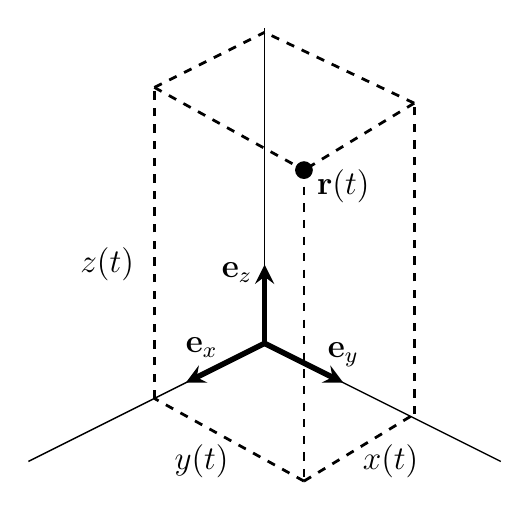
\begin{tikzpicture}
        \usetikzlibrary{shapes.arrows}
        \draw[black, line width=0.5pt] (0,0) -- (0,4.0);
        \draw[black, line width=0.5pt] (0,0) -- (3.0,-1.5);
        \draw[black, line width=0.5pt] (0,0) -- (-3.0,-1.5);
        
        \draw[black, -stealth, line width=2pt] (0,0) -- (0,1.0);
        \draw[black, -stealth, line width=2pt] (0,0) -- (1.0,-0.5);
        \draw[black, -stealth, line width=2pt] (0,0) -- (-1.0,-0.5);
        
        \filldraw (0.5,2.2) circle (3pt);
        \draw[black, dashed, line width=1pt] (0.5,2.2) -- (0.5,-1.75);
        
        \draw[black, dashed, line width=1pt] (0.5,-1.75) -- (1.9,-0.9);
        \draw[black, dashed, line width=1pt] (0.5,-1.75) -- (-1.4,-0.7);

        \draw[black, dashed, line width=1pt] (1.9,-0.9) -- (1.9,3.05);
        \draw[black, dashed, line width=1pt] (-1.4,-0.7) -- (-1.4,3.25);
        \draw[black, dashed, line width=1pt] (-1.4,3.25) -- (0.5,2.2);
        \draw[black, dashed, line width=1pt] (1.9,3.05) -- (0.5,2.2);
        \draw[black, dashed, line width=1pt] (1.9,3.05) -- (0.0,3.95);
        \draw[black, dashed, line width=1pt] (-1.4,3.25) -- (0.0,3.95);

        \node[black] at (-2,1.0) {\large$z(t)$};
        \node[black] at (-0.8,-1.5) {\large$y(t)$};
        \node[black] at (1.6,-1.5) {\large$x(t)$};

        \node[black] at (1.0,2.0) {\large$\mathbf{r}(t)$};
        
        \node[black] at (1.0,-0.15) {\large$\mathbf{e}_y$};
        \node[black] at (-0.8,-0.05) {\large$\mathbf{e}_x$};
        \node[black] at (-0.35,0.9) {\large$\mathbf{e}_z$};
      \end{tikzpicture}
    \end{center}
    \caption{Standard basis $\{\mathbf{e}_x, \mathbf{e}_y, \mathbf{e}_z\}$ in ${}^3\mathbb{R}$ and the
      coordinates in terms of this basis $x(t)$, $y(t)$, and $z(t)$.}
    \label{pic:stand}
  \end{figure}
\end{minipage}
\hfill\begin{minipage}{0.47\linewidth}
  \begin{figure}[H]
    \begin{center}
      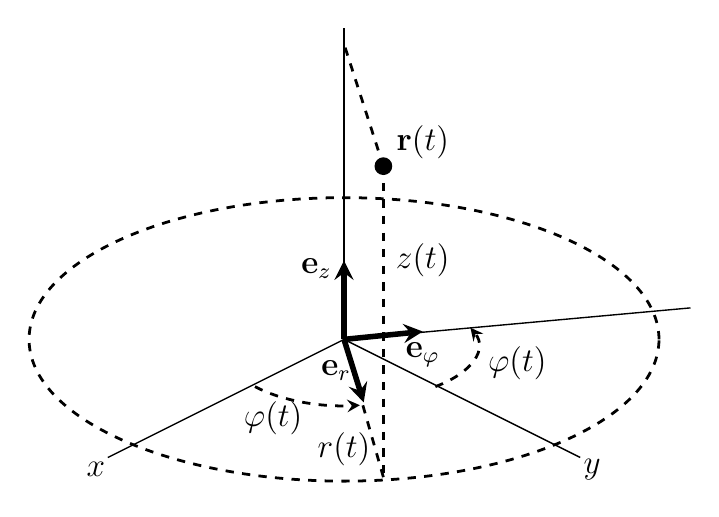
\begin{tikzpicture}
        \usetikzlibrary{shapes.arrows}
        \draw[black, line width=0.5pt] (0,0) -- (0,3.95);
        \draw[black, line width=0.5pt] (0,0) -- (3.0,-1.5);
        \draw[black, line width=0.5pt] (0,0) -- (-3.0,-1.5);

        \filldraw (0.5,2.2) circle (3pt);
        \draw[black, dashed, line width=1pt] (0.5,2.2) -- (0.5,-1.75);
        \draw[black, dashed, line width=1pt] (0.5,-1.75) -- (0,0);
        \draw[black, dashed, line width=1pt] (0.5,2.2) -- (0,3.75);
        
        \draw[black, -stealth, line width=2pt] (0,0) -- (0,1.0);
        \draw[black, -stealth, line width=2pt] (0,0) -- (0.25,-0.8);
        \draw[black, -stealth, line width=2pt] (0,0) -- (1.0,0.1);

        \draw[black, line width=0.5pt] (0,0) -- (4.4,0.4);
        
        \draw[black, dashed, line width=1.0pt] (0,0) ellipse (4 and 1.8);

        \draw[black, -stealth, dashed, line width=1pt] (-1.13,-0.6) arc(220:277:1.5 and 0.675);

        \draw[black, -stealth, dashed, line width=1pt] (1.16,-0.6) arc(-50:20:1.5 and 0.675);
        
        \node[black] at (1.0,1.0) {\large$z(t)$};
        \node[black] at (-0.9,-1.0) {\large$\varphi(t)$};
        \node[black] at (2.2,-0.3) {\large$\varphi(t)$};
        \node[black] at (0,-1.4) {\large$r(t)$};

        \node[black] at (1.0,2.5) {\large$\mathbf{r}(t)$};
        
        \node[black] at (-0.1,-0.4) {\large$\mathbf{e}_r$};
        \node[black] at (1.0,-0.2) {\large$\mathbf{e}_\varphi$};
        \node[black] at (-0.35,0.9) {\large$\mathbf{e}_z$};

         \node[black] at (-3.15,-1.65) {\large$x$};
         \node[black] at (3.15,-1.65) {\large$y$};
       \end{tikzpicture}
    \end{center}
    \caption{Cylindrical basis $\{\mathbf{e}_r, \mathbf{e}_\varphi, \mathbf{e}_z\}$ and the
      coordinates in terms of this basis $r(t)$ and $z(t)$, and the angle $\varphi(t)$.}
    \label{pic:cyl}
  \end{figure}
\end{minipage}

\pagebreak


\noin{\bf 1.}  

\vspace{20pt}

\noin{(a)} Express the velocity $\mathbf{\dot r}(t) $ of $\mathbf{r} \in {}^3\mathbb{R}$ in
Figure~\ref{pic:stand} in terms of the standard basis vectors
$\{\mathbf{e}_x, \mathbf{e}_y, \mathbf{e}_z\}$ and the coordinates $x$, $y$, and $z$. Additionally,
describe $\mathbf{\dot r}$ in Figure~\ref{pic:cyl} in terms of the cylindrical basis vectors
$\{\mathbf{e}_r, \mathbf{e}_\varphi, \mathbf{e}_z\}$, their time derivatives, and the coordinates $r$,
and $z$.

%  % Question 1(a)
{
	\vspace*{-10pt}
	%Do not change the height of this box. Your work must fit inside it.
	
	\makenonemptybox{150pt}{
    \begin{align}
      \text{In the standard basis: }& \mathbf{r}(t) = x(t) \mathbf{e}_x + y(t) \mathbf{e}_y + z(t) \mathbf{e}_z\\
      \mathbf{\dot r}(t) &= \dot x \mathbf{e}_x + x \dot{\mathbf{e}_x} + \dot y \mathbf{e}_y + y \dot{\mathbf{e}_y} + \dot z \mathbf{e}_z + z \dot{\mathbf{e}_z}\\
      \text{Since }& \mathbf{e}_x, \mathbf{e}_y, \mathbf{e}_z \text{ are constant, } \dot{\mathbf{e}_x} = \dot{\mathbf{e}_y} = \dot{\mathbf{e}_z} = 0\\
      \therefore \mathbf{\dot r}(t) &= \dot x \mathbf{e}_x + \dot y \mathbf{e}_y + \dot z \mathbf{e}_z\\
      \text{In the cylindrical basis: }& \mathbf{r}(t) = r(t) \mathbf{e}_r + z(t) \mathbf{e}_z\\
      \mathbf{\dot r}(t) &= \dot r \mathbf{e}_r + r \dot{\mathbf{e}_r} + \dot z \mathbf{e}_z + z \dot{\mathbf{e}_z}\\
      \text{Since }& \mathbf{e}_z \text{ is constant, } \dot{\mathbf{e}_z} = 0\\
      \therefore \mathbf{\dot r}(t) &= \dot r \mathbf{e}_r + r \dot{\mathbf{e}_r} + \dot z \mathbf{e}_z
    \end{align}

	%%% Your work goes here! 

	}
}
      


\noin{(b)} Determine the transformation matrix $\mathbf{P}$ mapping the standard basis to the
cylindrical basis:
$$\veccoll{\mathbf{e}_r}{\mathbf{e}_\varphi}{\mathbf{e}_z} = \mathbf{P}
\veccoll{\mathbf{e}_x}{\mathbf{e}_y}{\mathbf{e}_z} $$


%Question 1(b)
{
	\vspace*{-10pt}
	%%% Do not change the height of this box. Your work must fit inside it.
	
	\makenonemptybox{300pt}{
    $$\mathbf{e_r} = \mathbf{e_x} \cos(\varphi) + \mathbf{e_y} \sin(\varphi)$$
    $$\mathbf{e_\varphi} = - \mathbf{e_x} \sin(\varphi) + \mathbf{e_y} \cos(\varphi)$$
    $$\mathbf{e_z} = \mathbf{e_z}$$
    Therefore, the transformation matrix $\mathbf{P}$ is
    $$
      \mathbf{P} = \begin{bmatrix}
        \cos(\varphi) & \sin(\varphi) & 0\\
        - \sin(\varphi) & \cos(\varphi) & 0\\
        0 & 0 & 1
      \end{bmatrix}
    $$

	%%% Your work goes here! 

	}
}


\pagebreak

\noin{\bf 2.} As mentioned in the \textit{preamble}, the vectors in the cylindrical basis have to be
time-dependent if the point $\mathbf{r} (t)$ is moving on a path over time $t$. Therefore, the first
time derivative (velocity) of the cylindrical basis vectors are not zero.  \bigskip

\noin{(a)} Consider the linear transformation defined by
$$ \veccoll{\mathbf{\dot e}_r}{\mathbf{\dot e}_\varphi}{\mathbf{\dot
    e}_z} = \mathbf{D} \veccoll{\mathbf{e}_r}{\mathbf{e}_\varphi}{\mathbf{e}_z},
\hspace{0.5cm}\text{with the notation } \frac{\mathrm{d}}{\mathrm{d}t}
\veccoll{\mathbf{e}_r}{\mathbf{e}_\varphi}{\mathbf{e}_z} = \veccoll{\frac{\mathrm{d}}{\mathrm{d}t} \mathbf{e}_r}{\frac{\mathrm{d}}{\mathrm{d}t} \mathbf{e}_\varphi}{\frac{\mathrm{d}}{\mathrm{d}t} \mathbf{e}_z} = \veccoll{\mathbf{\dot e}_r}{\mathbf{\dot e}_\varphi}{\mathbf{\dot
    e}_z}$$

\noindent Determine the transformation matrix $\mathbf{D}$ for this transformation.
\medskip

\noindent \textit{Hint:} Start with the expression of the transformation in Question 1(b). Remember
also that $\varphi = \varphi(t)$ is time-dependent.


%Question 2(a)
{
	\vspace*{-10pt}
	%%% Do not change the height of this box. Your work must fit inside it.
	
	\makenonemptybox{450pt}{
    $$ \dot{\mathbf{e}_r} = \frac{d}{dt} (\mathbf{e}_x \cos(\varphi) + \mathbf{e}_y \sin(\varphi)) = - \mathbf{e}_x \sin(\varphi) \dot \varphi + \mathbf{e}_y \cos(\varphi) \dot \varphi$$
    $$ \dot{\mathbf{e}_\varphi} = \frac{d}{dt} (- \mathbf{e}_x \sin(\varphi) + \mathbf{e}_y \cos(\varphi)) = - \mathbf{e}_x \cos(\varphi) \dot \varphi - \mathbf{e}_y \sin(\varphi) \dot \varphi$$
    $$ \dot{\mathbf{e}_z} = 0$$
    Therefore, the transformation matrix from standard basis to the time derivative of the cylindrical basis is:
    $$ \mathbf{T}_{\dot{c} s} = \begin{bmatrix}
      - \sin(\varphi) \dot \varphi & \cos(\varphi) \dot \varphi & 0\\
      - \cos(\varphi) \dot \varphi & - \sin(\varphi) \dot \varphi & 0\\
      0 & 0 & 0
    \end{bmatrix}$$
    To get the transformation matrix from the cylindrical basis to the time derivative of the cylindrical basis, 
    we can multiply the $\mathbf{T}_{\dot{c} s}$ to a matrix that transforms the standard basis to the cylindrical basis.
    P is the change of base matrix from the standard basis to the cylindrical basis, 
    therefore the inverse of P is the change of base matrix from the cylindrical basis to the standard basis:
    $$ \mathbf{D} = \mathbf{T}_{\dot{c} s} \mathbf{P}^{-1} $$
    $$
      \mathbf{P} = \begin{bmatrix}
        \cos(\varphi) & \sin(\varphi) & 0\\
        - \sin(\varphi) & \cos(\varphi) & 0\\
        0 & 0 & 1
      \end{bmatrix}
    $$
    $$
    \Rightarrow
      \mathbf{P}^{-1} = \begin{bmatrix}
        \cos(\varphi) & - \sin(\varphi) & 0\\
        \sin(\varphi) & \cos(\varphi) & 0\\
        0 & 0 & 1
      \end{bmatrix}
    $$
    $$
    \mathbf{D} = \mathbf{T}_{\dot{c} s} \mathbf{P}^{-1}
      = \begin{bmatrix}
        - \sin(\varphi) \dot \varphi & \cos(\varphi) \dot \varphi & 0\\
        - \cos(\varphi) \dot \varphi & - \sin(\varphi) \dot \varphi & 0\\
        0 & 0 & 0
      \end{bmatrix}
      \begin{bmatrix}
        \cos(\varphi) & - \sin(\varphi) & 0\\
        \sin(\varphi) & \cos(\varphi) & 0\\
        0 & 0 & 1
      \end{bmatrix}
      = \begin{bmatrix}
        0 & \dot \varphi & 0\\
        - \dot \varphi & 0 & 0\\
        0 & 0 & 0
      \end{bmatrix}
    $$

    %%% Your work goes here!

	}
}
\pagebreak

\noin{\bf 2.} As mentioned in the \textit{preamble}, the vectors in the cylindrical basis have to be
time-dependent if the point $\mathbf{r} (t)$ is moving on a path over time $t$. Therefore, the first
time derivative (velocity) of the cylindrical basis vectors are not zero.  \bigskip

\noin{(b)} Determine the first time derivative $\frac{\mathrm{d}}{\mathrm{d}t}\mathbf{r} = \mathbf{\dot r}$ of
$\mathbf{r} \in {}^3\mathbb{R}$ expressed in the cylindrical basis from Question 1(a). For that, use the
transformation calculated in Question 2(a) and express $\mathbf{\dot r}$ as a linear combination of
$\mathbf{e}_r$, $\mathbf{e}_\varphi$, and $\mathbf{e}_z$.

%Question 2(b)
{
	\vspace*{-10pt}
	%%% Do not change the height of this box. Your work must fit inside it.
	
	\makenonemptybox{200pt}{
    From matrix $\mathbf{D}$, we have:
    $$ \dot{\mathbf{e}_r} = \dot \varphi \mathbf{e}_\varphi $$
    $$ \dot{\mathbf{e}_\varphi} = - \dot \varphi \mathbf{e}_r $$
    Therefore, the first time derivative of $\mathbf{r}$ in the cylindrical basis is:
    $$ \mathbf{\dot r}(t) = \dot r \mathbf{e}_r + r \dot{\mathbf{e}_r} + \dot z \mathbf{e}_z = \dot r \mathbf{e}_r + r \dot \varphi \mathbf{e}_\varphi + \dot z \mathbf{e}_z $$


	%%% Your work goes here! 
          
	}
}

\noin{(c)} Determine the second time derivative
$\frac{\mathrm{d}}{\mathrm{d}t} \mathbf{\dot r} = \mathbf{\ddot r}$ of
$\mathbf{r} \in {}^3\mathbb{R}$ expressed in the cylindrical basis from Question 1(a). Use the
transformation calculated in Question 2(a) and express $\mathbf{\ddot r}$ as a linear combination of
$\mathbf{e}_r$, $\mathbf{e}_\varphi$, and $\mathbf{e}_z$.

%Question 2(c)
{
	\vspace*{-10pt}
	%%% Do not change the height of this box. Your work must fit inside it.
	
	\makenonemptybox{200pt}{
    \begin{align}
      \mathbf{\ddot r} &= \frac{d}{dt} (\dot r \mathbf{e}_r + r \dot \varphi \mathbf{e}_\varphi + \dot z \mathbf{e}_z) = \ddot r \mathbf{e}_r + \dot r \dot{\mathbf{e}_r} + \dot r \dot \varphi \mathbf{e}_\varphi + r \ddot \varphi \mathbf{e}_\varphi + r \dot \varphi \dot{\mathbf{e}_\varphi} + \ddot z {\mathbf{e}_z}\\
      &= \ddot r \mathbf{e}_r + 2 \dot r \dot \varphi \mathbf{e}_\varphi + r \ddot \varphi \mathbf{e}_\varphi - r {\dot \varphi}^2 \mathbf{e}_r + \ddot z {\mathbf{e}_z}\\
      &= (\ddot r - r {\dot \varphi}^2) \mathbf{e}_r + (2 \dot r \dot \varphi + r \ddot \varphi) \mathbf{e}_\varphi + \ddot z \mathbf{e}_z
    \end{align}
    

	%%% Your work goes here! 
          
	}
}



\pagebreak

\noin{\bf 3.} We are now using the cylindrical basis to study a moth circling a light source in the
dark. We can describe the path of the moth as a logarithmic spiral towards the light source. The
moth flys with a constant angle $\alpha$ and with constant path velocity $v$ in the direction of the
light source (see Figure~\ref{pic:moth}).

  \begin{figure}[H]
    \begin{center}
      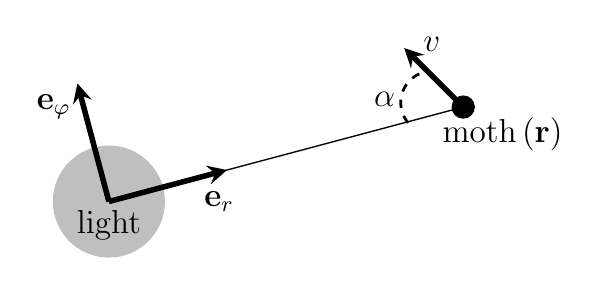
\begin{tikzpicture}
        \usetikzlibrary{shapes.arrows}

        \filldraw[black] (0.0,0.0) circle (1pt);
        \filldraw[lightgray, line width=0.5pt] (0.0,0.0) circle (20pt);
                
        \draw[black, -stealth, line width=2pt] (0,0) -- (-0.4,1.5);
        \draw[black, -stealth, line width=2pt] (0,0) -- (1.5,0.4);

        \draw[black, line width=0.5pt] (0,0) -- (1.5*3,0.4*3);
        \filldraw[black] (1.5*3,0.4*3) circle (4pt);
        \draw[black, -stealth, line width=2pt] (1.5*3,0.4*3) -- (1.5*3-0.75,0.4*3+0.75);

        \draw[black, dashed, line width=1pt] (1.5*3-0.7,0.4*3-0.2) arc(220:100:0.4 and 0.4);

        \node[black] at (1.4,0) {\large$\mathbf{e}_r$};
        \node[black] at (-0.7,1.2) {\large$\mathbf{e}_\varphi$};
        \node[black] at (0,-0.3) {\large light};
        \node[black] at (5.0,0.85) {\large moth\,(\textbf{r})};
        \node[black] at (3.5,1.3) {\large$\alpha$};
        \node[black] at (4.1,2.0) {\large$v$};        
       \end{tikzpicture}
    \end{center}
    \caption{View from above of a moth circling a light source at hight $z = \text{const.} = 0$.}
    \label{pic:moth}
  \end{figure}
\medskip

\noin{(a)} Calculate the acceleration of the moth in $\mathbf{e}_r$ direction by using your result
from Question 2(c). For that, break down the velocity components in Figure~\ref{pic:moth} for
$\mathbf{\dot r}$ using the cylindrical basis.


%Question 3(a)
    
    {
	\vspace*{-10pt}
	%%% Do not change the height of this box. Your work must fit inside it.
	
	\makenonemptybox{230pt}{
    $$ \dot{\mathbf{r}} = -v\cos(\alpha) \mathbf{e}_r + v\sin(\alpha) \mathbf{e}_\varphi = \dot r \mathbf{e}_r + r \dot \varphi \mathbf{e}_\varphi + \dot z \mathbf{e}_z$$
    $$ \Rightarrow \dot r = -v\cos(\alpha), r \dot \varphi = v\sin(\alpha)$$
    Since $v$ and $\alpha$ are constants, $\ddot r = 0$ and $ \frac{d}{dt} (r \dot \varphi) = \dot r \dot \varphi + r \ddot \varphi = 0$. 
    Using the result from Question 2(c), we have:
    $$ \mathbf{\ddot r} = (\ddot r - r {\dot \varphi}^2) \mathbf{e}_r + (2 \dot r \dot \varphi + r \ddot \varphi) \mathbf{e}_\varphi + \ddot z \mathbf{e}_z = - r {\dot \varphi}^2 \mathbf{e}_r + \dot r \dot \varphi \mathbf{e}_\varphi + 0 \mathbf{e}_z$$
    $$ r = \int -v\cos(\alpha) \,dt = -v\cos(\alpha)t + C $$
    $$ r \dot{\varphi}^2 = \frac{(r \dot \varphi)^2}{r} = \frac{v^2 \sin^2(\alpha)}{-v\cos(\alpha)t + C} = \frac{v \sin(\alpha) \tan(\alpha)}{-t + C_1} $$
    ($C$ is the initial radius that the moth starts at.)\\
    Therefore the acceleration of the moth in $\mathbf{e}_r$ direction is:
    $$ \mathbf{a}_r = - r {\dot \varphi}^2 \mathbf{e}_r = \frac{v \sin(\alpha) \tan(\alpha)}{t + C_2} \mathbf{e}_r$$
    Where $C_2$ is a constant of integration.
          %%% Your work goes here! 

	}
}

\noin{(b)} Interprete your result from Question 3(a). Discuss what happens if the moth gets close to
the light source. How do you explain your observation that a moth drifts away at a critical distance
from the light source and starts its approach again? No additional calculations are necessary.

%Question 3(b)
    
    {
	\vspace*{-10pt}
	%%% Do not change the height of this box. Your work must fit inside it.
	
	\makenonemptybox{150pt}{
    By the linear relationship between time and the orbiting radius, $ r = -v\cos(\alpha)t + C $,
    and that the moth's initial radius is greater than zero; moth will approach the light in the $\mathbf{e}_r$ direction and will
    eventually reach it at the origin. By the logarithmic spiral motion of the moth, the radius of the moth's motion is dependent on $\phi$, and
    as the moth approaches the light, it's orbiting frequency will tend toward infinity at some finite time; this is the critical time.
    Therefore, the moth's critical distance is 0 at some finite time for which radius will become negative and the angle of motion will
    tend waya from the light source. After the critical point, the moth will never approach the light source again as the radius $r$ becomes more negative with time.
          %%% Your work goes here! 

	}
}
      
\end{document}
